\chapter{Conception}
\label{ch:conception}

All the components of the system or how they are connected to each other are described in this chapter.
The map of the pins is also described in this chapter.

% ---------------------------------------------------------
\section{Core application}
\label{conception:core-application}

The core application is the application that is installed on the Raspberry Pi and she's responsible for the communication with the devices and the clients.
This application is written in C++ and uses the WiringPi library to communicate with the devices and REST API with web sockets to communicate with the clients.

\subsection{Packages}
\label{conception:core-application:packages}

The core application is divided into two parts.

The first part is the communication with the devices.
This part is to simplify the usage of the devices and hide the complexity of the communication.
This part uses the WiringPi library to communicate with the devices.

The second part is the communication with the clients.
This part is the REST API and the web socket.
The REST API is used to configure the devices and the web socket is used to send the data to the clients.
He uses the first part to communicate with the devices.

There is also a third part that is a singleton that stores the state of the application.
This part is used by the device’s part to store the information and by the REST API to send the information to the clients.

\begin{figure}[ht]
  \centering
  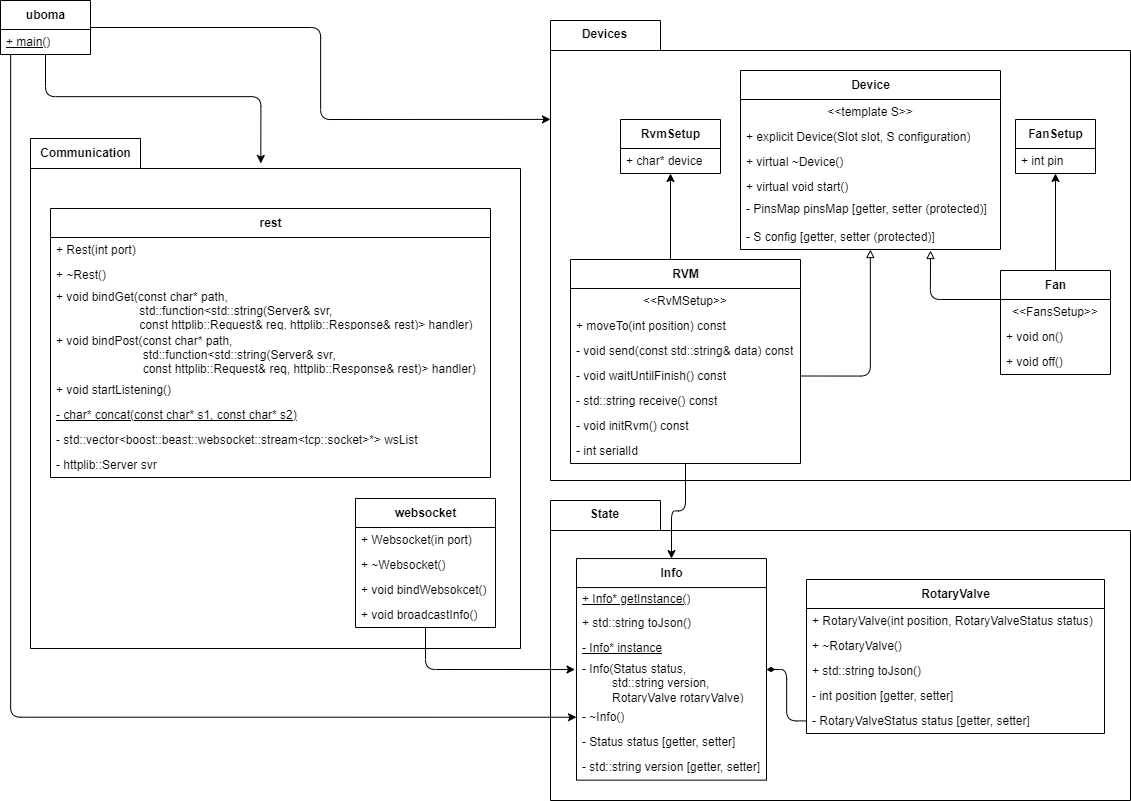
\includegraphics[width=1\textwidth]{img/conception_packages.drawio.png}
  \caption{Core application packages}
  \label{fig:conception:core-application:packages:illustration}
\end{figure}

The figure \ref{fig:conception:coreApplication:packages:illustration} illustrate the packages of the core application.
There is no link between the communication and the devices because the action of the route of the REST API are directly defined in the uboma.

\subsection{Threads}
\label{conception:core-application:threads}

The core application must manage many tasks at the same time, so it uses threads to do that.
The main thread starts to initialize all the devices and the route of the REST API.
The handling of the REST API is done in a thread that will create a new thread for each request.
The main thread will also listen to the web socket and create a new thread for each new client.
The figure \ref{fig:conception:coreApplication:threads:illustration} illustrate the relation of each thread.

\begin{figure}[ht]
  \centering
  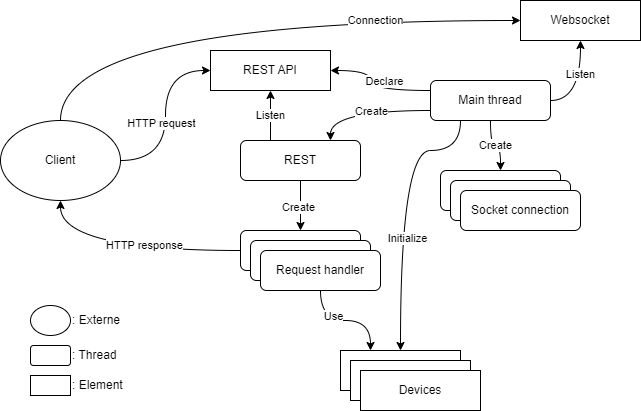
\includegraphics[width=1\textwidth]{img/conception_threads.drawio.png}
  \caption{Threads illustration}
  \label{fig:conception:core-application:threads:illustration}
\end{figure}

\subsection{Register routes}
\label{conception:core-application:register-routes}
 To register the routes of the REST API, the core application must provide a route and the handler to the class `Rest`.
 This class will set default header to match with the \acrfull{cors} policy and register the route with the handler.

 \begin{figure}[ht]
  \centering
  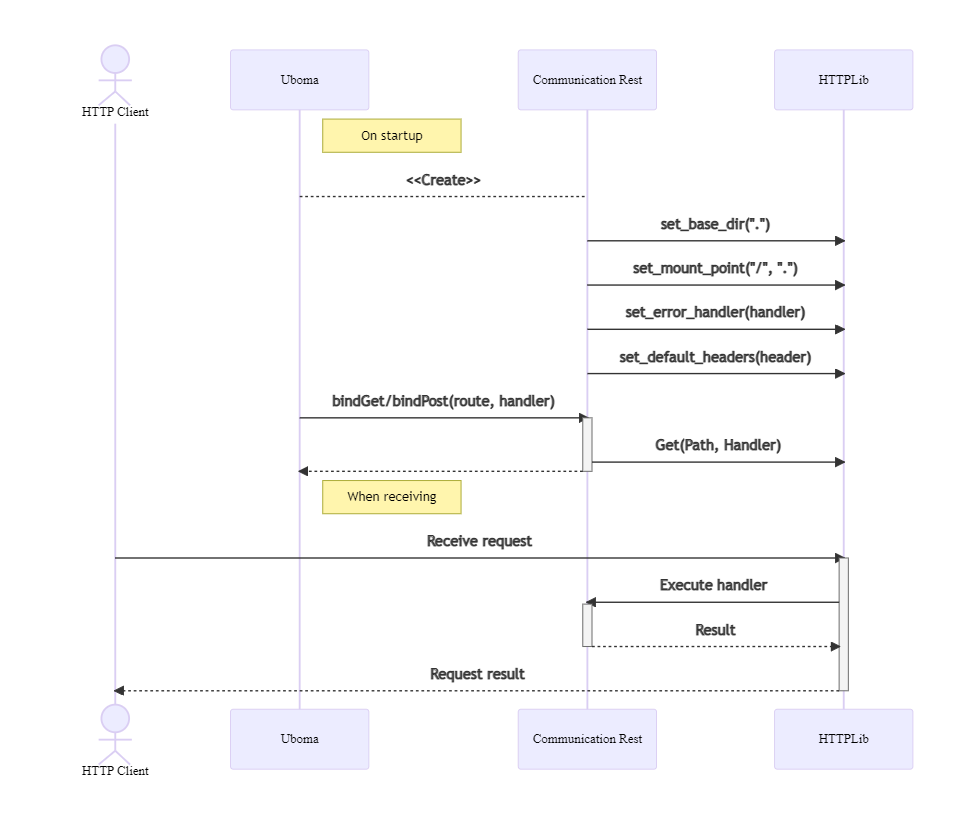
\includegraphics[width=1\textwidth]{img/conception_routes.drawio.png}
  \caption{Register routes sequence}
  \label{fig:conception:core-application:register-routes:illustration}
 \end{figure}

The figure \ref{fig:conception:core-application:register-routes:illustration} illustrate the sequence to register a route and what is made when a request is received.
The class `Rest` surcharge the `HTTPLib` class to add the default header and use thread to listen to the requests.
When a request is received, the class will call the handler.


% ---------------------------------------------------------
\section{Client application}
\label{conception:client-application}

The client application is the application that will be used by the user to interact with the core application.
This application is written in Flutter and use REST API and web socket to communicate with the core application.
Flutter is a framework to create a cross-platform application and it can easily be compiled for Android, iOS, Windows, Linux and MacOS.

\subsection{Mockup}
\label{conception:client-application:mockup}

This is the mockup of the application, the first page of the figure \ref{fig:conception:client-application:mockup:illustration} is the home page.
This page will allow us to do a classic dispense and show the status of the whole system.
The second page is the advanced page.
Each device can be configured and the all his data can be seen.

\begin{figure}[h]
  \centering
  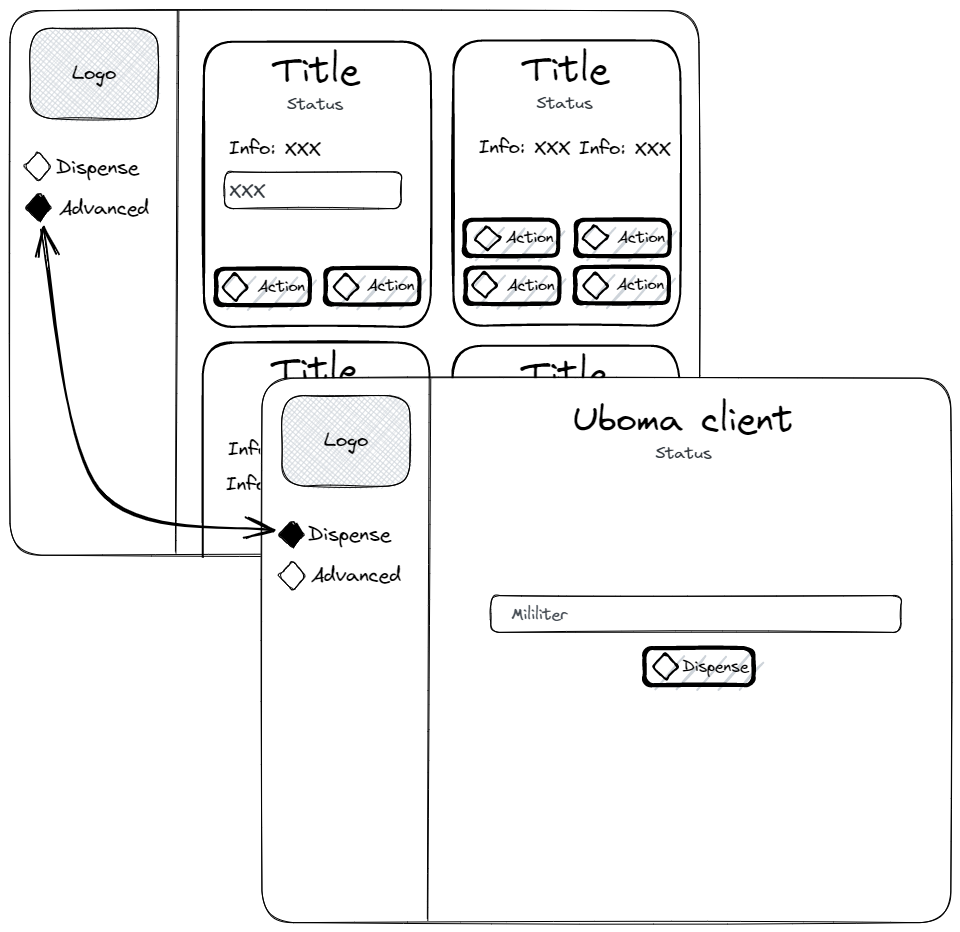
\includegraphics[width=0.65\textwidth]{img/conception_clientApp.excalidraw.png}
  \caption{Mockup of the application}
  \label{fig:conception:client-application:mockup:illustration}
\end{figure}

The cards represent the devices and they will be adapted to each device.

\subsection{Architecture}
\label{conception:client-application:architecture}

The client application follows the \acrfull{mvvm} pattern.
This pattern is used to separate the logic of the application from the view.
The data are managed by a repository which uses the REST API to communicate with the core application.
There \acrshort{mvvm} is a little bit violated because the view is directly linked to the repository.

\begin{figure}[h]
  \centering
  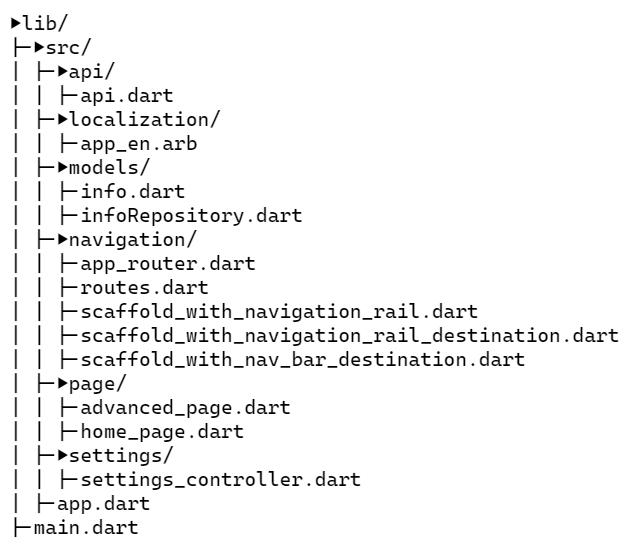
\includegraphics[width=0.55\textwidth]{img/conception_architecture.excalidraw.png}
  \caption{Client application architecture}
  \label{fig:conception:client-application:architecture:illustration}
\end{figure}

The figure \ref{fig:conception:client-application:architecture:illustration} shows the architecture of the client application.
The view is defined in the `page` folder and they are the `Info` stored in the repository.
The files in `localization` are used to translate the application.
To add a new language, a new file must be created in this folder.
The navigation has its own folders and there are multiple files because the application is responsive and the navbar is moving to the bottom on mobile.



\section{Pins}
\label{sec:pins}

The number of the pins of the library WiringPi isn't the same as the number in schema of Mikroe for the shield.
The following table \ref{tab:pin-map} shows the correspondence between the pins of the library WiringPi and the pins of the shield.

% \usepackage{tabularray}
\begin{longtblr}[
    caption = {Pins map},
    label = {tab:pin-map},
  ]{
    row{1} = {c},
    row{2} = {c},
    cell{1}{1} = {r=2}{},
    cell{1}{2} = {r=2}{},
    cell{1}{3} = {r=2}{},
    cell{1}{4} = {r=2}{},
    cell{1}{5} = {c=3}{},
    vline{1-6} = {1-2}{},
    vline{6-8} = {2}{},
    vline{1,8} = {1-41}{},
    hline{1,3-42} = {-}{},
    hline{2} = {5-7}{},
  }
  \textbf{\# } & \textbf{Name } & \textbf{WiringPi } & \textbf{Shield }   & \textbf{Slot } &              &              \\
                     &                &                    &                    & \textbf{One}   & \textbf{Two} & \textbf{Ext} \\
  1                  & 3.3v           &                    &                    &                &              &              \\
  2                  & 5v             &                    &                    &                &              &              \\
  4                  & 5v             &                    &                    &                &              &              \\
  5                  & SCL1           & 9                  & GPIO3/I2C-SCL      & SCL            & SCL          & SCL          \\
  6                  & 0v             &                    &                    &                &              &              \\
  7                  & GPIO7          & 7                  & GPIO4              &                &              &              \\
  8                  & TxD            & 15                 & GPIO14/UART-TX     & TX             & TX           & TX           \\
  9                  & 0v             &                    &                    &                &              &              \\
  10                 & RxD            & 16                 & GPIO15/UART-RX     & RX             & RX           & RX           \\
  11                 & GPIO0          & 0                  & GPIO17             &                &              &              \\
  12                 & GPIO1          & 1                  & GPIO18/PWM1        & PWM            &              &              \\
  13                 & GPIO2          & 2                  & GPIO27             &                &              & INT          \\
  14                 & 0v             &                    &                    &                &              &              \\
  15                 & GPIO3          & 3                  & GPIO22             &                &              & RST          \\
  16                 & GPIO4          & 4                  & GPIO23/CS2         &                &              & CS           \\
  17                 & 3.3v           &                    &                    &                &              &              \\
  18                 & GPIO5          & 5                  & GPIO24             &                &              &              \\
  19                 & MOSI           & 12                 & GPIO10/SPI-MOSI~ ~ & MOSI           & MOSI         & MOSI         \\
  20                 & 0v             &                    &                    &                &              &              \\
  21                 & MISO           & 13                 & GPIO9/SPI-MISO~ ~  & MISO           & MISO         & MISO         \\
  22                 & GPIO6          &                    & SPIO25/DRDY~ ~     &                &              &              \\
  23                 & SCLK           & 14                 & GPIO11/SPI-SCK~ ~  & SCK            & SCK          & SCK          \\
  24                 & CE0            & 10                 & GPIO8/CS0          & CS             &              &              \\
  25                 & 0v             &                    &                    &                &              &              \\
  26                 & CE1            & 11                 & GPIO7/CS1~ ~       &                & CS           &              \\
  27                 & SDA0           & 30                 & -                  &                &              &              \\
  28                 & SCL0           & 31                 & -                  &                &              &              \\
  29                 & GPIO21         & 21                 & GPIO5              & RST            &              &              \\
  30                 & 0v             &                    &                    &                &              &              \\
  31                 & GPIO22         & 22                 & GPIO6~ ~           & INT            &              &              \\
  32                 & GPIO26         & 26                 & GPIO12             &                & RST          &              \\
  33                 & GPIO23         & 23                 & GPIO13/PWM2        &                & PWM          &              \\
  34                 & 0v             &                    &                    &                &              &              \\
  35                 & GPIO24         & 24                 & -                  &                &              &              \\
  36                 & GPIO27         & 27                 & GPIO16/PWM1~ ~     &                &              & PWM          \\
  37                 & GPIO25         & 25                 & GPIO26             &                & INT          &              \\
  38                 & GPIO28         & 28                 & GPIO20/FAN~ ~      &                &              &              \\
  39                 & 0v             &                    &                    &                &              &              \\
  40                 & GPIO29         & 29                 & -                  &                &              &
\end{longtblr}

